% Use British English. 

\documentclass{jimis} 

% Packages
\usepackage[utf8]{inputenc}
\usepackage{array}
\usepackage{pgfplots}
\usepackage{graphicx}
\usepackage{grffile}
\usepackage[left,modulo,pagewise]{lineno}

% Comments
\newcommand{\frb}[1]{\textbf{/* #1 (Fariba) */}}   
\newcommand{\jxk}[1]{\textbf{/* #1 (Jérôme) */}}   
\newcommand{\para}[1]{\smallskip\noindent\textbf{#1}}

% header
\title{ The Problem of Action at a Distance in Networks and the Emergence of Preferential Attachment from Triadic Closure }
% title suggestion: explaining the emergence of scaling using hidden variable model
%%\title{ Action at a Distance in Networks }

\author[*1]{Jérôme KUNEGIS}
\author[1,2]{Fariba KARIMI}
\author[1]{SUN Jun}
\affil[1]{University of Koblenz--Landau, Germany} 
\affil[2]{GESIS -- Leibniz-Institut für die Sozialwissenschaften, Germany} 
% corresponding author with his/her email
\corrauthor{kunegis@uni-koblenz.de}

%% Information provided by JIMIS:
%ISSN
% DOI 
\doi{XXXX}{000}
% reviewing process: first date = submission, second date = acceptance 
\review{Month/Day/Year}{Month/Day/Year}
% Volume and Year of the issue
\publication{N}{YYYY}

%% Information provided by the Editors:
% Issue Title 
\issue{Graphs \& Social Systems}
% List of k Editors
\editors{First-name-$1$ Family-name-$1$, First-name-$2$ Family-name-$2$, First-name-$k$ Family-name-$k$...}

\begin{document}

\maketitle

\linenumbers

\abstract{
In this paper, we characterise the notion of preferential
attachment in networks as action at a distance, and argue that it can
only be an emergent phenomenon -- the actual mechanism by which networks
grow always being the closing of triangles.
After a review of the concepts of triangle closing and preferential
attachment, we present our argument, as well as a simplified model in
which preferential attachment can be derived mathematically from
triangle closing. 
}

\keywords{Networks, preferential attachment, triangle closing, action at
  a distance}

\section{Introduction}
%\strut
%\vspace{-4ex}
Many natural and man-made phenomena are networks -- i.e., ensembles of
interconnected entities.  To understand such structures is to understand
their creation, their evolution and their decay.  In fact, many models
have been described for the evolution of networks, for the simple reason
that such a large amount of systems consist of interconnected parts. 
Rules for the 
evolution of networks can be broadly classified into two classes: those
postulating local growth, and those postulating global growth.  An
example for a mechanism of local growth is triangle closing: When two
people become friends because they have a common friend, then a new
triangle is formed, consisting of three persons.  This tendency of
networks to form triangles is a natural model not only for social
networks, but for almost all types of networked data.  For instance, if
Alice likes a movie and Bob is friends with Alice, Bob might also come
to like that movie.  In this case, the triangle consists of two persons
and one movie.  In general, networks can contain any type of object
being connected by many different types of connections, and thus many
different types of such triangle closings are possible.  We call this
type of growth \emph{local} because it only depends on the immediate
neighbourhood of the two connected nodes; the rest of the network does
not play a role.

\begin{figure}
  \centering
  \subfigure[Triangle closing]{
    \includegraphics[width=0.18\textwidth]{pics/Triadic closure}
  }
  \subfigure[Preferential attachment]{
    \includegraphics[width=0.47\textwidth]{pics/Preferential attachment}
  }
  \caption{
    \label{fig:illustration}
    The two network growth mechanisms considered in this article:
    triangle closing and preferential attachment.  In both models, new
    edges appear (shown as dashed lines), based on the network
    environment of the current graph. (a)~Triangle closing:  an edge
    is more likely to appear between nodes that have common neighbours,
    (2)~Preferential attachment:  An edge is more likely to appear
    between nodes that have high degree. 
  }
\end{figure}

On the other hand, there is preferential attachment.  When, for
instance, two people become friends with each other, not because they
have a common friend, or go to the same class, but because they are both
popular.  Given two very popular persons, i.e.\ with many friends, it is
more likely that they will become friends, than that two unpopular
people will become friends, all else being equal.  This phenomenon is
referred to as preferential attachment.  Preferential attachment is an
often-used strategy to predict new connections, not only in social
networks: a frequent movie-goer is much more likely to watch a popular
film, than someone who almost never goes out to the movies watching an
obscure film almost nobody knows or has seen.  These types of statements
seem obviously true and indeed they are used widely in application
systems: recommender systems give a big preference to popular movies,
search engines give higher weight to well-connected web pages, and
Facebook or Twitter will make a point to show you pictures that already have many
likes.  In that sense, preferential attachment is true empirically, and
has been verified many times in experiments.  Then, what is problematic with
preferential attachment?  Is it not always correct?  No, we are not
claiming that preferential attachment is wrong.  What we argue is that
preferential attachment is never a primitive phenomenon, but always a
derived phenomenon, emerging as a result of more basic network evolution
rules.

So, if preferential attachment is not a fundamental network evolution
mechanism, what \emph{makes} a fundamental network mechanism, and which
fundamental network evolution rules are then fundamental?  We will
present in this paper arguments for the thesis that
only the principle of triangle closing is fundamental, all forms of
preferential attachment being derived from it. 
To give an
argument in favour of our thesis, we will first review basic notions of
networks and network evolution models, and then review 
preferential attachment, proposing various mechanisms by which
it can arise from triangle closing, a fundamental notion in the
evolution of networks. 

\section{Networks}
The statement \emph{everything is a network} has become a cliché because
it is true.  Social networks, knowledge networks, information networks,
communication networks -- many papers in the field of network science
motivate their use by enumerating fields in which they play a central
role.  Biological networks, molecules, lexical networks, Feynman
diagrams -- hardly a scientific field exists in which networks do not play
a fundamental role.  Instead of giving a hopelessly incomplete
enumeration of examples, we will simply refer the reader to the
introductory section of our Handbook of Network Analysis
\citep{konect:handbook}, in case she wishes to convince herself of
this fact.  In case this is not enough, we may point to the existence of entire
fields of research incorporating the word \emph{network} that have emerged
in the last decade: network science \citep{network-science,newman2010networks}, web science
\citep{web-science} and others \citep{tiropanis2015}.
Then, why \emph{is} everything a network?
To find an answer, it is instructive to consider the field of machine
learning. 
Most classical machine learning algorithms deal with
datasets consisting of data points, each consisting of the same
features.  Mathematically, we may model such a dataset as a set of
points in a space whose dimensions are the individual features \citep{vector-space-model}.
This formalism is very powerful, and still constitutes the backbone of many
machine learning and data mining methods to this day.  The standard
formulation of classification, clustering and other learning problems
all rely on the set-of-points-in-a-space model. However, not all do.
While the set of words contained in text documents are well represented
by the \emph{bag of words} model, a social network is not.  We may try to
represent a social network as a bag of friends, but this
representation is very unsatisfactory:  each person has a set of
friends, but the model does not consider the fact that a person
contained in one of these bags is the same person as one
\emph{having} a bag of friends.  Thus, the vector space model cannot
find connections such as ``the friend of my friend'' -- it can only find
``a person that has the same friend as me''.  In other words, the vector
space model disconnects the role of \emph{having friends} and that of
\emph{being a friend}.  Instead, the natural way to represent
friendships is as a network.  Using a network model, the symmetry of the
friend relationship is included automatically in the model, and
relationships such as \emph{the friend of my friend} arise as the
natural way to create new edges in the network, i.e., triangle closing.
In fact, we will argue that this is the only way new edges can be created in a network, and
that other models are merely consequences of it, such as preferential
attachment. 

\section{Preferential Attachment}
Preferential attachment, also referred to by the phrase ``the rich get
richer'', or as the Matthew effect,
is observed in many social networks.  In other words,
who has many friends, will get more new friends than who has few.  Movies
that have been seen by many people will be seen by more people than
movies that have not.  Websites that have been linked to many times will
receive more new links because of this.  These statements seem true, and
indeed, they are true empirically for many different network types
\citep{kunegis:preferential-attachment}. 

In fact, preferential attachment is the basis for a whole class of
network models.  The most basic of these, the model of Albert-László
Barabási and Réka Albert (\citeyear{barabasi-albert}), describes the growth of a network
as follow:  Start with a small graph, and at each step, add a node, and
connect that node to $k$ existing nodes with a probability proportional
to the number of neighbours for each existing node.  In the limit where
many nodes have been added in that way, the network tends to become
\emph{scale-free}, i.e.\ tends to have a distribution of neighbour counts
that follow a power law.  Since power law degree
distributions are observed in many natural networks, the usual conclusion
is that preferential attachment is correct. 

Preferential attachment is thus undeniably real.  Why then, are we
arguing against it?
The reason is that preferential attachment cannot be a fundamental
driving force for tie creation. 
How are two nodes, completely unconnected from each
other, be supposed to choose to connect with each other?  How can two
completely disconnected nodes even \emph{know} of each others existence?
This is a fundamental problem with all nonlocal interactions.  For
instance, the classical theory of gravitation as defined and used by
Isaac Newton (\citeyear{newton}) includes nonlocal interactions.  In that
theory, two masses exert a force on each other, regardless of their
position.  While the force decreases with distance, it is always
nonzero, and instantaneous.  The conceptual problem with this type of
interaction has been identified even by Newton himself
\citep{hesse}.  In modern physics, Newton's formalism is replaced by more
precise theories that do not include any action at a distance.  The
theory of general relativity as defined by Albert Einstein in 1916 for
instance, only includes local interaction in the from of the Einstein
field equations \citep{einstein}.  Einstein's general relativity is
thus free from any problematic \emph{action at a distance}, and has been
verified at many experimental scales.  This is also true for
other types of physical interactions -- instead of a force that acts at
a distance between matter particles, quantum field theory models
\emph{bosons} that connect 
particles.  In fact, such interactions can be represented by Feynman
diagrams: graph-like representations of particles in which edges are
particles and nodes are interactions -- any interacting particles must
be connected in one diagram, directly or indirectly.  In this light, we
may interpret preferential attachment as a theory that is true
superficially, but must be explained by an underlying phenomenon.
Specifically, an underlying phenomenon that does not rely on action at a
distance.  As this phenomenon, we propose the known mechanism of
triangle closing.

\section{Triangle Closing}
How do we make new friends?  By meeting the friends of our friends.
This represents a triangle formed by us, our previous friend and our
new friend.  What if we meet our new friend in another way -- maybe at a
party, or a concert, or at work \ldots\ in any case there is always
\emph{some} element in common. If we meet our new friend at a party, then
we are both connected to the party, and by modelling the party as a node
in our network, that new friendship is indeed created by the closing of
a person--person-party triangle.  Of course, we may continue to ask how
our connection to the party 
arose.  After all, we did not come to a random party or to a
random party with many guests.  No -- we came to the party because a
friend invited us, or for any other reason, as long as there is some
connection.  This game of connections can be played to any
desired degree of precision.  Maybe we \emph{really} went from door to
door until we found a party with many people.  But then, how did we get
from door to door?  We surely have started somewhere, likely near to our
home, and have then gone on to the next door, and to the next door, and
so on.  In doing this, we have only followed links:  We are connected to
our home by living there;  our home is connected to the neighbouring
house, which itself is connected to the next house, and so on. 
This example is of course exaggerated, but serves to illustrate the
principle:  in order for a new edge to appear, a path has to exist from
one node to another; this can go over node representing any type of
entity, and these nodes may be visible or hidden. 
All in 
all, there is no escaping the principle of triangle closing.  However we
arrived at the party, it must have been by a series of triangle
closings.  

Thus, triangles fulfil our expected as a fundamental mechanism of
network growth, as it is purely local. 
However, we cannot deny the existence of preferential attachment, for which
we must now find suitable explanations. 

\section{Explanations}
In recommender systems, such as that used on web sites that recommend movies to
watch, preferential attachment is often taken as a solution to the cold
start problem.  The cold start problem in recommender systems refers to
the situation in which a user has not yet entered any information about
herself, and thus triangle closing cannot be used to recommend her
anything.  If the user has watched only a single movie, then we can find
similar movies and recommend them.  If a user has added only a single
friend, then we can take movies liked by that friend and recommend them.
But if the user is completely new, as has no friends and no ratings yet,
then this strategy will not work.  How then, do recommender systems give
recommendations to new users?  The solution is simple: they recommend
the most popular items.  If you subscribe to Twitter, you will be
recommended popular accounts to follow.  If you subscribe to Last.fm,
you will be recommended popular music.  For these sites, this strategy
is better than not recommending anything, and in fact is a form of
preferential attachment: Create, or rather recommend, links to nodes
with many neighbours.  How can we interpret this in terms of triangle
closing?  If a node has no connections yet, then surely it cannot
acquire new nodes by triangle closing.  How then will a node ever
acquire new edges, if it starts without neighbours?  The answer is that
a node does not start without any neighbours.  Everything is connected.
A child when it is born does not start without connections; it is
already connected to its parents and to its birthplace.  Likewise a
user on the Web never starts from scratch: every page has a referrer,
and thus the user can be connected to another website.  Even if the
referring web page is not known, there has to be a referrer.  If a user
types in a URL by hand, she has to have taken it somewhere: maybe a
friend gave it to her, maybe she read it
in a magazine, on a billboard, or on a truck \ldots\ in all cases, the
newly created connection is not created \emph{ex nihilo} -- it is created
by triangle closing.

The explanation for preferential attachment thus lies in hidden nodes:
Nodes that make indirect connections between things, but do not appear
in the modelled system.  On Facebook for instance, many new
friendships are created between people who do not have common friends.
These new friendships seemingly appear without the help of triangle
closing.  However, that is always due to the fact that Facebook does not know
everything.  Some people are simply not on Facebook, which means that if
I meet a new friend through a friend of mine that is not on Facebook and
then connect with my new friend via Facebook, then from the point of
view of Facebook a new edge was created without triangle
closing.
But
that is only true because Facebook does not know my initial friend.  If
it did, it could correctly infer the new friendship via triangle
closing.  Thus, any two nodes in a network can potentially be linked,
even if they do not share common neighbours \emph{in the network at
  hand}, because they may share a hidden common neighbour.  
The same argumentation applies to hidden nodes that represent
non-actors, such as classes, hometowns, parties, etc. 

If any edge can be explained by hidden nodes, how can it then be that
edges connecting nodes with high degree are observed more often? 
Imagine a network, for instance a social
network.  Call this the known network.  Then imagine a certain number of
nodes outside of that 
network, that are connected at random to the nodes in the known
network.  Call these the unknown nodes.   How many common neighbours do
two members of the known network 
have outside of the known network?  Without knowing the distribution of
hidden edges, this question cannot be answered.  But consider that
triangle closing acts not only on known--unknown--known triangles, but
also on known--known--unknown triangles.  Starting with an equal
probability for all known--unknown edges, performing triangle closing
will lead to the creation of known--known--unknown triangles.  The newly
created known--unknown edges can then be combined with other
unknown--known edges to perform, again, triangle closing, leading to new 
known--known edges.  The result are new edges in the observed social
network, with a probability proportional to the number of the initial
known node's neighbours.  
Thus, preferential attachment emerges as a necessary consequence of
iterated triangle closing, if hidden nodes are admitted.
The next section will make this heuristic argument precise. 

\section{Derivation}
This section gives an exemplary derivation of a simplified model that we
introduce to illustrate our explanation, in 
which preferential 
attachment arises as a consequence of triangle closing in the presence
of hidden nodes.  The given scenario is very general and may be generalised
easily for instance by considering multiple node or edge types.  
In this model, we distinguish two types of nodes:  visible nodes in the set $V$,
and hidden nodes in the set $W$.  We will assume that there is a given,
fixed number of visible nodes $|V|$, and a possibly very large number of
hidden nodes $|W|$.  In particular, we will consider the limit $|W|
\rightarrow \infty$. 

%% \begin{figure}
%%   \centering
%%   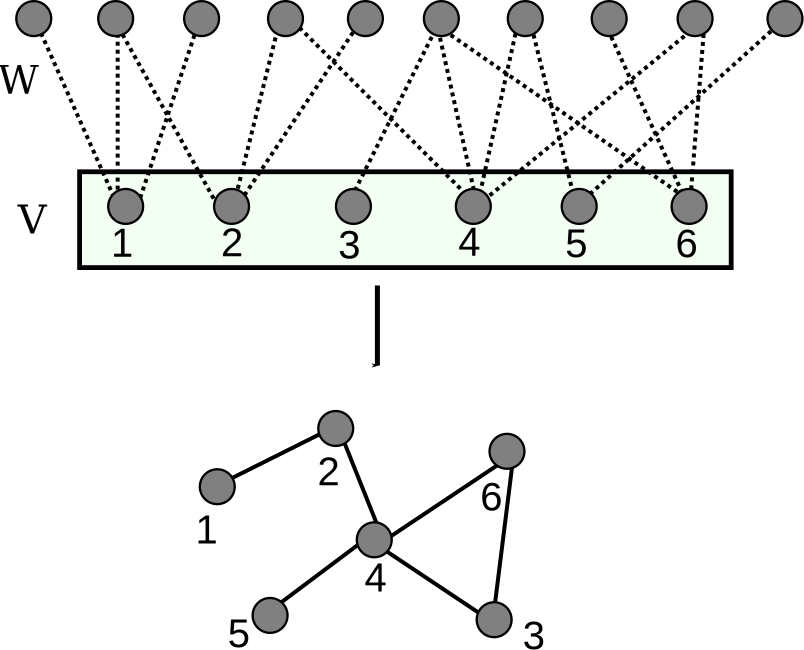
\includegraphics[width=0.5\textwidth]{pics/derivation_illust}
%%   \caption{
%%     \label{fig:derivation}
%%     A toy example of the model. $G=(V \cup W, E)$ is a bipartite network in which only nodes in set $V$ are visible. Nodes in set $W$ are invisible and are connected to nodes in set $V$ by invisible edges that is shown by dashed lines. Projecting the visible set of nodes in a unipartite graph results in preferential attachment. 
%%   }
%% \end{figure}

Let $G=(V \cup W, E)$ be a bipartite network in which only the nodes $V$
and their degree are visible, the edges $E$ and the nodes $W$ are not
visible.  Assuming that two nodes in $V$ connect with a probability
proportional the number of common nodes they have.  Edge between nodes
in $V$ will not be considered, except for their effect on the degree of
nodes in $V$.  Likewise, edges between nodes in $W$ need not be
considered.  Thus, the considered network $G$ is bipartite. 
We will use the convention that $n = |W|$, and the degree of a node $x$ is
denoted by $d(x)$. 
Seeing only nodes in $V$ and their degree, preferential attachment can
be observed in the following way. 

In order to make our derivation, we need to make two assumptions:
\begin{itemize}
  \item The edges of the graph are randomly distributed between possible
    node pairs.
  \item The typical degree of nodes are significantly smaller than the
    number of nodes, i.e., $d(x) \ll n$.  This is precise when $n$ goes
    to infinity.  
\end{itemize}

Let $u,v \in V$ be two nodes of the network.  Under the assumption that
the edges are distributed randomly in the graph, the probability $p$
that $u$ and $v$ are connected can be derived combinatorically by
considering the number of configurations in which the two nodes do not
share a common neighbor.  Given that $u$ and $v$ have degree $d(u)$ and
$d(v)$ respectively, the total number of configurations for the edges
connected to the nodes is
\begin{align*}
  {{n} \choose {d(u)}} {{n} \choose {d(v)}}.
\end{align*}
Out of those, the number of configurations in which the neighbours of
the two nodes are disjoint is given by
\begin{align*}
  {{n} \choose {d(u)}} {{n - d(u)} \choose {d(v)}}.
\end{align*}
Thus, the probability that the two nodes share a common neighbour is
given by 
\begin{align*}
  p &= 1 - \frac
  {{{n} \choose {d(u)}} {{n - d(u)} \choose {d(v)}}}
  {{{n} \choose {d(u)}} {{n} \choose {d(v)}}}
  = 1 - \frac
  {{{n - d(u)} \choose {d(v)}}}
  {{{n} \choose {d(v)}}}.
\end{align*}
We now use the falling factorial to express binomial coefficients, i.e.,
\begin{align*}
  n^{\underline{a}} = n(n-1)(n-2)\cdots(n-a+1). 
\end{align*}
The falling factorial has the property that in the limit where $a$ is
constant and $n$ goes to infinity, we have
\begin{align*}
  \lim_{n \rightarrow \infty} \frac {n^{\underline{a}}}{n^a} = 1
\end{align*}
and also,
\begin{align*}
  {n \choose a} = \frac {n^{\underline{a}}} {a!}, 
\end{align*}
and thus
\begin{align*}
  p = 1 - \frac
  {(n - d(u))^{\underline{d(v)}} d(v)!}
  {d(v)! n^{\underline{d(v)}}} 
  = \frac
  {(n - d(u))^{\underline{d(v)}}}
  {n^{\underline{d(v)}}}
\end{align*}
with the limit
\begin{align*}
  p = 1 - \frac
  { (n - d(u))^{d(v)} }
  { n         ^{d(v)} }
  = 1 - \left( 1 - \frac {d(u)} {n} \right)^{d(v)}
\end{align*}
and using the limit $n \rightarrow \infty$ again:
\begin{align*}
  p = \frac {d(u)d(v)} {n}. 
\end{align*}
It thus follows that $p \sim d(u)d(v)$, i.e., the probability of the
nodes $u$ and $v$ being connected is proportional to both $u$ and $v$.
Thus, preferential attachment is a consequence of the triangle closing
model. 
Preferential attachment itself then leads to a scale-free degree
distribution, as per Barabási and Albert \citeyearpar{barabasi-albert}. 

\section{Related Work}
The debate over the nature of preferential attachment mechanism dates
back to the 1960s, when the economist H.~Simon defended the role of
randomness and the mathematician B.~Mandelbrot defended the role of
optimization \citep{barabasi2012network}. The concept of preferential
attachment is also able to explain the nature of scale-free degree
distribution in biological networks such as metabolic networks
\citep{jeong2000large} and protein networks
\citep{jeong2001lethality}. There are various suggestions to explain the
nature of preferential attachment for instance by introducing  hidden variable
models in which nodes possess an intrinsic fitness to other nodes in
unipartite \citep{boguna2003class} or bipartite networks
\citep{kitsak2011}. In a recent \emph{Nature} paper, Papadopoulos et
al. proposed a model based on geometric optimization of homophily space
\citep{papadopoulos2012popularity}. However, in these models, 
triadic closure is not defined as the main principle for the formation
of edges.  

Triadic closure, a tendency to connect to friend of a friend
\citep{rapoport1953spread}, has been observed undeniably in many social
networks such as friendship at university
\citep{kossinets2006empirical}, scientific collaboration
\citep{newman2001clustering} and World Wide Web
\citep{adamic1999small}. The concept of triadic closure was first
suggested by German sociologist Georg Simmel
\citeyear{simmel1950sociology} and later on popularized by Fritz Heider
and Mark Granovetter as the theory of cognitive Balance in which if two
individuals feel the same way about the an object/person, they seek
closure by closing the triad between themselves
\citep{heider2013psychology}.  
Since the classic preferential attachment model lacks to explain the number of clusters in many social networks, many attempts have been make to include triadic closure to the model \citep{holme2002growing,vazquez2003growing}, in
which nodes with certain probability connect based on the principle of
triadic closure.  These works have shown that the scaling law for the
degree distribution and clustering coefficient can be reproduced based
on these models \citep{klimek2013triadic}.

Hence,the scale-free nature of networks and the abundance of triangles beg for
a more fundamental explanation.  Moreover, the observable part of the
systems is not necessarily completely representative for the entire
system.  Networks are generally multi-layered or multiplex, in which some
layers can be hidden or simply not possible to observe
\citep{kivela2014multilayer}.  For instance, the creation of a new Facebook tie
can be caused by attending the same class, sharing the same hobby or
living in a same neighborhood,  which is hidden from the observable
data.  Consequently, these ``focal'' points contribute to the tie
creation known as ``focal closure'' and need to be considered in
modeling realistic networks, as argued by Kossinets and Watts
\citeyearpar{kossinets2006empirical}.  
  


%A model of hidden variables in bipartite network is defined in \citep{kitsak2011}.
% http://arxiv.org/pdf/1104.3184v2.pdf

\section{Discussion}
The status of a mechanism as \emph{fundamental} is not clear cut.  When
a phenomenon is explained by another, more fundamental phenomenon, then
we can consider it as derived.  But how can we be sure that a phenomenon
is not explained by a more basic phenomenon?  What does it mean for a
phenomenon to be fundamental?  Just as physics cannot declare one theory
to be final, network science cannot declare one network growth mechanism
to be final.  Thus, individual instances of triangle closing can for
instance be explained by several layers of triangle closing, just as in
physics a direct interaction can be explained by a new mediating
particle.  In the end however, this applies only to specific instances
of triangle closing, as it replaces them with other, more detailed
instances of triangle closing.  Thus triangle closing \emph{does} play a
fundamental role in network models, only that we cannot state which
triangle closing is the fundamental one.  In the end, the only judge of
the validity of a model remains the experiment, and in practice, used
models do not have to be fundamental -- recommenders and information
retrieval systems have had enough success by applying 
preferential attachment directly.

\bibliographystyle{jimis}
\bibliography{nopref}

\end{document}

